\section{Evaluation}
\subsection{Data Preparation and Metrics}
To do the evaluation, we select corpus on six well-known libraries. They are Java Development Kit (JDK), Android, GWT, Joda-Time, Hibernate, and XStream. These libraries were selected to generate the corpus for other research works (\cite{8453132,Subramanian:2014:LAD:2568225.2568313}). To generate corpus, we select 1000 highest stars Java projects from Github (\cite{id:Github}), which have most files used API from libraries in Table \ref{tbl:DataPreparation}. For each Java project, InvocMap parses each Java source files by an the Train ASTVisitor module on Figure \ref{fig:ApproachOverview}. We apply our solution using Phrasal \cite{Green2014}.The number of methods we collect is shown in Table \ref{tbl:DataPreparation}. 
\begin{table}[]
\small
\centering
\caption{Statistics on Corpus}
\begin{tabular}{|l|l|}
\hline
\textbf{Library }  & \textbf{Num of methods} \\ \hline
JDK       & 820386         \\ \hline
GWT       & 170435         \\ \hline
Joda-Time & 91072          \\ \hline
Android   & 312822         \\ \hline
Hibernate & 149887         \\ \hline
Xstream   & 159170         \\ \hline
\end{tabular}

\label{tbl:DataPreparation}
\end{table}

\subsubsection{Training Configuration} To train the SMT model, we use a high-end computer with core-i7 Intel processor and use 32 GB of memory. We allocate Phrasal with phrase length equals to 7. The total training time requires about 6 hours.

\subsubsection{Test Configuration}
We evaluate the ability of translation from a sequence of method names to ASTs in level 3 of abstraction. We simulate 3 configurations sequences of method names regarding to its local context defined in Table \ref{tbl:Config2}. 

\begin{table}[]
\small
\centering
\caption{3 Testing Configurations for Developers}
\begin{tabular}{|l|Q|}
\hline
                     & \textbf{Meaning / Example    }                                                                                              \\ \hline
\multirow{2}{*}{\textbf{Config 1}} & Only method name                                                               \\ \cline{2-2} 
                     &  println                                                                   \\ \hline
\multirow{2}{*}{\textbf{Config 2}} &  method name and variables                                                                                       \\ \cline{2-2} 
                         & println 10 5                                        \\ \hline
\multirow{2}{*}{\textbf{Config 3}} & method name, variables and some suggested words                                                                                 \\ \cline{2-2} 
               &      println 10 + 5       
                     \\ \hline
Expected &                          
System.out.println(\#+\#)
\\ & Params: int and int     
                     \\ \hline
\end{tabular}

\label{tbl:Config2}
\end{table}

We can see the local context provided for method names is increasing from configurations at level 1 to level 3. At level 1, the input for translation contains only method names with the code context in the source language for translation. It simulates the case that developers write a list of method names inside the code environment. At level 2, information about partial class name of types of local entities is attached along with each method names. This case simulates the case developers remember and write method name and local variables (s)he needs to implement the MI but (s)he doesn't remember the structure of AST. At level 3, each method names in the source language will be attached the information about local entities and half of words appeared inside the MI. This case simulates the case that developers remember some words inside the MI along with local entities. In Table \ref{tbl:Config2}, at level 3 developer input \texttt{println} as method name, 2 integers as variables and an operator \texttt{+}. The input for predicting the MI is \texttt{int\#var int\#var println\#identifier +\#term}. And the translation engine needs to return as MI respected to \texttt{println\#identifier}.

\subsubsection{Metrics}
We evaluate the correct inference of method names. Information about tokens of method name can be recognized by the annotation \texttt{\#identifier} for the source, and the expected results can be recognized by prefix \texttt{"E-Total"} of tokens in the target. We use Precision and Recall as 2 metrics for the evaluation. We category cases of predicting tokens of method name: True Positive (TP)- means the prediction is correct; False Positive (FP) - means the expected expression is in the training corpus but the translated expression is different and False Negative (FN) - means the expected expression is out of vocabulary (OOV). Out of Vocabulary is the case that the method name token does not in the corpus (Out of Source - OOS) or the expected expression token does not appear in the target corpus (Out of Target - OOV). 
 
\subsection{Research Question (RQ) 1: How InvocMap can perform to predict the implementation with Intrinsic Data?}

  \begin{table*}[t]
  \small
  \centering
  \caption{Intrinsic Evaluation Result on Github projects}
\begin{tabular}{|l|l|l|l|l|l|l|l|l|l|}
\hline
          &  \multicolumn{9}{c|}{\textbf{Intrinsic Evaluation with Configuration 1}}           \\
\hline
\textbf{Library}   & \textbf{Correct} & \textbf{Incorrect} & \textbf{OOSource} & \textbf{OOTarget} & \textbf{OOVoc}  & \textbf{Total}   & \textbf{Precision} & \textbf{Recall}  & \textbf{F1-Score} \\ \hline
GWT       & 39635   & 22318     & 3082     & 28440    & 31522  & 93475   & 63.98\%   & 55.70\% & 59.55\%  \\ \hline
Joda-Time & 27364   & 10608     & 51       & 1692     & 1743   & 39715   & 72.06\%   & 94.01\% & 81.59\%  \\ \hline
JDK       & 1053330 & 540997    & 3691     & 390626   & 394317 & 1988644 & 66.07\%   & 72.76\% & 69.25\%  \\ \hline
Android   & 471347  & 91753     & 5654     & 48662    & 54316  & 617416  & 83.71\%   & 89.67\% & 86.58\%  \\ \hline
Hibernate & 53319   & 25305     & 4787     & 34090    & 38877  & 117501  & 67.82\%   & 57.83\% & 62.43\%  \\ \hline
Xstream   & 4671    & 1692      & 70       & 2949     & 3019   & 9382    & 73.41\%   & 60.74\% & 66.48\%  \\ \hline
Total     & 1649666 & 692673    & 17335    & 506459   & 523794 & 2866133 & 70.43\%   & 75.90\% & 73.06\%  \\ \hline
          & \multicolumn{9}{c|}{\textbf{Intrinsic Evaluation with Configuration 2}} \\
\hline
\textbf{Library}   & \textbf{Correct} & \textbf{Incorrect} & \textbf{OOSource} & \textbf{OOTarget} & \textbf{OOVoc}  & \textbf{Total}   & \textbf{Precision} & \textbf{Recall}  & \textbf{F1-Score} \\ \hline
GWT       & 53042                                     & 8911      & 3082     & 28440    & 31522  & 93475   & 85.62\%   & 62.72\% & 72.40\%  \\ \hline
Joda-Time & 29028                                     & 8944      & 51       & 1692     & 1743   & 39715   & 76.45\%   & 94.34\% & 84.45\%  \\
\hline
JDK       & 1347221                                   & 247064    & 3691     & 390668   & 394359 & 1988644 & 84.50\%   & 77.36\% & 80.77\%  \\
\hline
Android   & 470725                                    & 92370     & 5654     & 48667    & 54321  & 617416  & 83.60\%   & 89.65\% & 86.52\%  \\
\hline
Hibernate & 63275                                     & 15345     & 4787     & 34094    & 38881  & 117501  & 80.48\%   & 61.94\% & 70.00\%  \\
\hline
Xstream   & 5145                                      & 1218      & 70       & 2949     & 3019   & 9382    & 80.86\%   & 63.02\% & 70.83\%  \\
\hline
Total     & 1968436                                   & 373852    & 17335    & 506510   & 523845 & 2866133 & 84.04\%   & 78.98\% & 81.43\%  \\
\hline
          & \multicolumn{9}{c|}{\textbf{Intrinsic Evaluation with Configuration 3}}        \\
\hline
\textbf{Library}   & \textbf{Correct} & \textbf{Incorrect} & \textbf{OOSource} & \textbf{OOTarget} & \textbf{OOVoc}  & \textbf{Total}   & \textbf{Precision} & \textbf{Recall}  & \textbf{F1-Score} \\ \hline
GWT       & 55510                                     & 6443      & 3082     & 28440    & 31522  & 93475   & 89.60\%   & 63.78\% & 74.52\%  \\
\hline
Joda-Time & 31394                                     & 6578      & 51       & 1692     & 1743   & 39715   & 82.68\%   & 94.74\% & 88.30\%  \\
\hline
JDK       & 1435424                                   & 158861    & 3691     & 390668   & 394359 & 1988644 & 90.04\%   & 78.45\% & 83.84\%  \\
\hline
Android   & 498708                                    & 64387     & 5654     & 48667    & 54321  & 617416  & 88.57\%   & 90.18\% & 89.36\%  \\
\hline
Hibernate & 65860                                     & 12760     & 4787     & 34094    & 38881  & 117501  & 83.77\%   & 62.88\% & 71.84\%  \\
\hline
Xstream   & 5516                                      & 847       & 70       & 2949     & 3019   & 9382    & 86.69\%   & 64.63\% & 74.05\%  \\
\hline
Total     & 2092412                                   & 249876    & 17335    & 506510   & 523845 & 2866133 & 89.33\%   & 79.98\% & 84.40\%  \\
\hline
\end{tabular}

\label{tbl:Intrinsic}
\end{table*}

We split the pairs of our parallel corpus for training and testing. We get 10\% of the data for testing and the other with training and do ten-fold cross-validation to test the ability of prediction on our full data set. In total, there are 2.86 Million of MIs collected from 1000 projects from Github \cite{id:Github}.
The evaluation result for intrinsic data is shown in Table \ref{tbl:Intrinsic}. We show that from configuration 1 to configuration 3, the F1 score increases from 73.06\% to 84.4\%. This seems to be feasible, since the fact that if we provide more local context information along with method names, the ability to predict correctly AST in level 3 for the translation model is better. We see one observation is that the number of Out of Vocabulary expressions are higher in percentage, cause decreasing in recall compare to the research work that applied Machine Translation for inferring Fully Qualified Name from incomplete code (\cite{8453132}). This is reasonable, since our work requires to infer the MI in level 3 of abstraction, which contains detail structure compared to output of \cite{8453132} as type information of MIs. 
\begin{figure}[]
        \center{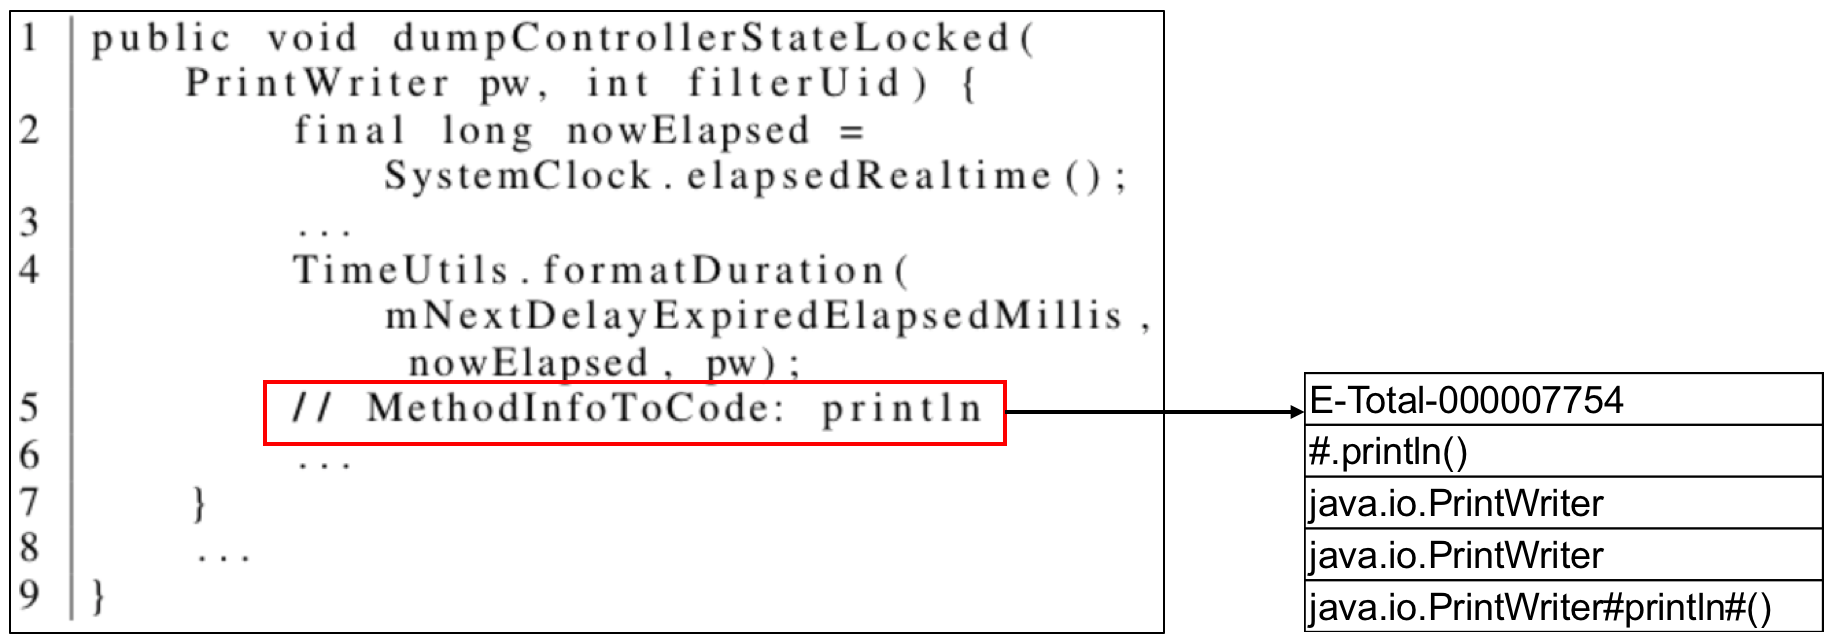
\includegraphics[width=\linewidth]
        {images/example_in.png}}
        \caption{\label{fig:example_in} Example of query in configuration 1 for code snippet in \cite{id:IntrinsicAndroidExample}}
      \end{figure}
We study an example in the Intrinsic Evaluation in Figure \ref{fig:example_in}. This example is a function collected from \cite{id:IntrinsicAndroidExample} from our corpus. The testing for intrinsic evaluation simulates the case developers input only \texttt{println} inside the code environment, the output of this case will be the implementation of \texttt{java.io.PrintWriter.println()} function. We can see that the surrounding code is useful to infer the correct expression. If we do not have the context information, which means developer input \texttt{println} in an empty method, the translated result will return the most popular MI, \texttt{System.out.println()}.

\subsection{RQ2: How well InvocMap can perform to predict the implementation with Extrinsic Data?}

To do this experiment, we collect the data as code snippets from Online Forums (\cite{id:StackOverflow,id:ProgramCreek,id:GeeksForGeeks}). To do this, a Software Engineer who has 5 years of experience in Java programming was hired to collect code snippets from 120 posts in Online Forums, with 20 posts for each library in Table \ref{tbl:DataPreparation}. Each code snippets are required to have the MIs of 6 libraries: JDK, Android, GWT, Joda-Time, Hibernate, and XStream. We run our Test ASTVisitor module to extract the source tokens with embedding MIs at 3 levels and use the SMT model learned from our parallel corpus for the prediction.

\begin{table*}[t]
\small
\centering
\caption{Extrinsic Evaluation Result on Online Forum Code Snippets}
\begin{tabular}{|l|l|l|l|l|l|l|l|l|l|}
\hline
          & \multicolumn{9}{c|}{\textbf{Extrinsic Evaluation with Configuration 1}}                             \\ \hline
\textbf{Library}   & \textbf{Correct} & \textbf{Incorrect} & \textbf{OOSource} & \textbf{OOTarget} & \textbf{OOVoc}  & \textbf{Total}   & \textbf{Precision} & \textbf{Recall}  & \textbf{F1-Score} \\ \hline
GWT       & 58      & 35        & 0        & 9        & 9     & 102   & 62.37\%   & 86.57\% & 72.50\%  \\ \hline
Joda-Time & 36      & 22        & 2        & 15       & 17    & 75    & 62.07\%   & 67.92\% & 64.86\%  \\ \hline
JDK       & 115     & 91        & 0        & 44       & 44    & 250   & 55.83\%   & 72.33\% & 63.01\%  \\ \hline
Android   & 51      & 42        & 0        & 13       & 13    & 106   & 54.84\%   & 79.69\% & 64.97\%  \\ \hline
Hibernate & 125     & 61        & 1        & 39       & 40    & 226   & 67.20\%   & 75.76\% & 71.23\%  \\ \hline
Xstream   & 44      & 6         & 0        & 14       & 14    & 64    & 88.00\%   & 75.86\% & 81.48\%  \\ \hline
Total     & 429     & 257       & 3        & 134      & 137   & 823   & 62.54\%   & 75.80\% & 68.53\%  \\ \hline
          & \multicolumn{9}{c|}{\textbf{Extrinsic Evaluation with Configuration 2}}                             \\ \hline
\textbf{Library}   & \textbf{Correct} & \textbf{Incorrect} & \textbf{OOSource} & \textbf{OOTarget} & \textbf{OOVoc}  & \textbf{Total}   & \textbf{Precision} & \textbf{Recall}  & \textbf{F1-Score} \\ \hline
GWT       & 88      & 5         & 0        & 9        & 9     & 102   & 94.62\%   & 90.72\% & 92.63\%  \\ \hline
Joda-Time & 53      & 5         & 2        & 15       & 17    & 75    & 91.38\%   & 75.71\% & 82.81\%  \\ \hline
JDK       & 177     & 29        & 0        & 44       & 44    & 250   & 85.92\%   & 80.09\% & 82.90\%  \\ \hline
Android   & 85      & 8         & 0        & 13       & 13    & 106   & 91.40\%   & 86.73\% & 89.01\%  \\ \hline
Hibernate & 138     & 48        & 1        & 39       & 40    & 226   & 74.19\%   & 77.53\% & 75.82\%  \\ \hline
Xstream   & 49      & 1         & 0        & 14       & 14    & 64    & 98.00\%   & 77.78\% & 86.73\%  \\ \hline
Total     & 590     & 96        & 3        & 134      & 137   & 823   & 86.01\%   & 81.16\% & 83.51\%  \\ \hline
          & \multicolumn{9}{c|}{\textbf{Extrinsic Evaluation with Configuration 3}}                             \\ \hline
\textbf{Library}   & \textbf{Correct} & \textbf{Incorrect} & \textbf{OOSource} & \textbf{OOTarget} & \textbf{OOVoc}  & \textbf{Total}   & \textbf{Precision} & \textbf{Recall}  & \textbf{F1-Score} \\ \hline
GWT       & 89      & 4         & 0        & 9        & 9     & 102   & 95.70\%   & 90.82\% & 93.19\%  \\ \hline
Joda-Time & 55      & 3         & 2        & 15       & 17    & 75    & 94.83\%   & 76.39\% & 84.62\%  \\ \hline
JDK       & 174     & 32        & 0        & 44       & 44    & 250   & 84.47\%   & 79.82\% & 82.08\%  \\ \hline
Android   & 82      & 11        & 0        & 13       & 13    & 106   & 88.17\%   & 86.32\% & 87.23\%  \\ \hline
Hibernate & 146     & 40        & 1        & 39       & 40    & 226   & 78.49\%   & 78.49\% & 78.49\%  \\ \hline
Xstream   & 50      & 0         & 0        & 14       & 14    & 64    & 100.00\%  & 78.13\% & 87.72\%  \\ \hline
Total     & 596     & 90        & 3        & 134      & 137   & 823   & 86.88\%   & 81.31\% & 84.00\%  \\ \hline
\end{tabular}

\label{tbl:Extrinsic}
\end{table*}

The result for extrinsic evaluation is shown in Table \ref{tbl:Extrinsic}. We see that with level 1, since the case that only method names are provided in the source language, our approach stills predict correctly 62.54\% in precision. With the configuration levels that developers add more information, the precision increases to 86.88\%. For each library, we achieved the highest accuracy on GWT and lowest on Hibernate with input as detail information like configuration 3. This result seems reasonable, since Hibernate is a bigger library compared to GWT but it is not as popular as JDK, causes the variety of ASTs for APIs in this library.




\subsection{RQ3: How well InvocMap can perform to predict ambiguous method names?}

In this evaluation, we analyze the relation of the expression prediction result relates to the number of mapping of each method name from the parallel corpus. We use data collected for the Intrinsic Evaluation with configuration 3, means each method names are embedded with local entities and local terms in the source language. The result is shown in Table \ref{tbl:Analyze1}.

\begin{table}[]
\small
\centering
\caption{Analyze Relation between Accuracy and Num of distinct mapping of Config 3}
\begin{tabular}{|l|l|l|l|l|l|}
\hline
              
\textbf{Num }& \textbf{1-10}        & \textbf{11-20}       & \textbf{21-50}       & \textbf{50-100}      & \textbf{\textgreater{}100}     \\
\textbf{of mapping }&         &        &        &       &      \\ \hline
\textbf{Percentage  }   & 12.30\%     & 4.20\%      & 5.96\%      & 4.90\%      & 72.64\%               \\ \hline
\textbf{Accuracy }      & \textbf{Prec}        & \textbf{Prec}        & \textbf{Prec}        & \textbf{Prec}        & \textbf{Prec}                  \\ \hline
GWT            & 96.58\%     & 86.83\%     & 88.71\%     & 86.89\%     & 86.59\%               \\ \hline
Joda-Time      & 93.38\%     & 89.64\%     & 76.19\%     & 69.43\%     & 74.11\%               \\ \hline
JDK            & 98.14\%     & 96.02\%     & 95.26\%     & 91.92\%     & 89.06\%               \\ \hline
Android        & 96.24\%     & 92.51\%     & 90.63\%     & 89.08\%     & 82.58\%               \\ \hline
Hibernate      & 92.61\%     & 87.60\%     & 87.50\%     & 85.47\%     & 78.98\%               \\ \hline
Xstream        & 97.78\%     & 91.01\%     & 78.81\%     & 81.02\%     & 80.80\%               \\ \hline
Total          & 96.47\%     & 93.07\%     & 92.05\%     & 89.41\%     & 87.68\%               \\ \hline
\end{tabular}

\label{tbl:Analyze1}
\end{table}
The result shows that from the number of method name that has more than 100 mappings in the parallel corpus are about 72\% of the total data. It proves the complexity of kinds of implementation for each method names. The total precision tends to decrease from 96.47 \% to 87.68\%. This proves the ability to generate expression from input queries.





